%% Enhanced Figure Index for HW-1 Paper
%% Auto-generated by generate_all_enhanced.py
%% Includes 9 comprehensive figures

\section{Figures}

%% ===== Main Figures =====

\begin{figure}[htbp]
  \centering
  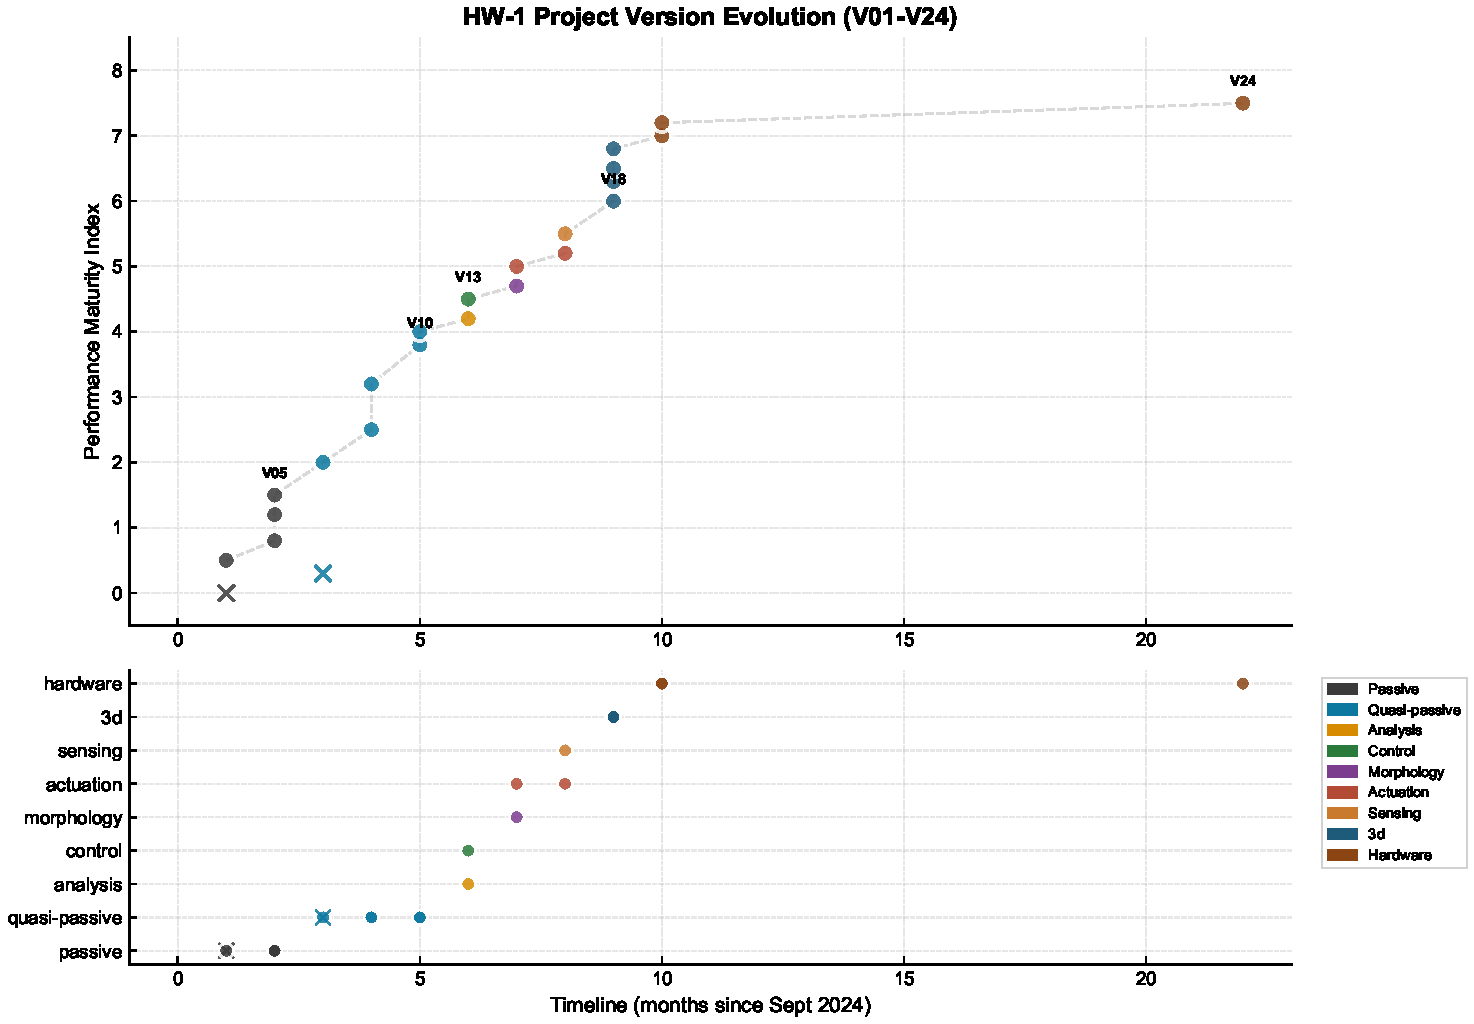
\includegraphics[width=\textwidth]{paper_figures/output/fig1_version_evolution.pdf}
  \caption{Version Evolution Timeline: Development progress from V01 (Compass Gait) to V24 (Sim-to-Real).
  Top panel shows performance maturity index progression. Bottom panel shows category distribution across versions.
  Key milestones: V05 (passive limit cycle proof), V10 (rolling foot), V13 (FSM control), V18 (3D stability), V24 (hardware deployment).}
  \label{fig:version_evolution}
\end{figure}

\begin{figure}[htbp]
  \centering
  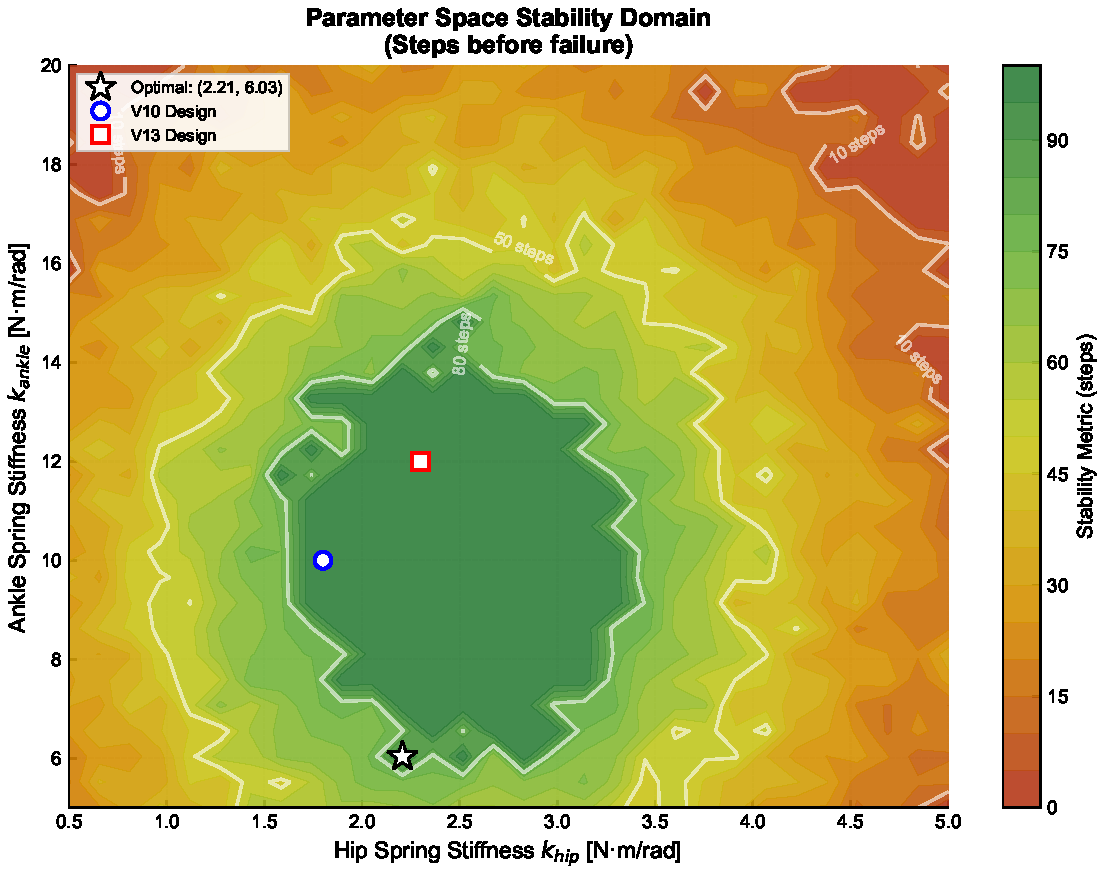
\includegraphics[width=0.85\textwidth]{paper_figures/output/fig2_stability_domain.pdf}
  \caption{Parameter Space Stability Domain: Heatmap showing gait stability (steps before failure) as a function of hip and ankle spring stiffness.
  White star indicates optimal parameters. Blue circle (V10) and red square (V13) show actual design choices.
  Contour lines mark stability thresholds at 10, 50, and 80 steps.}
  \label{fig:stability_domain}
\end{figure}

\begin{figure}[htbp]
  \centering
  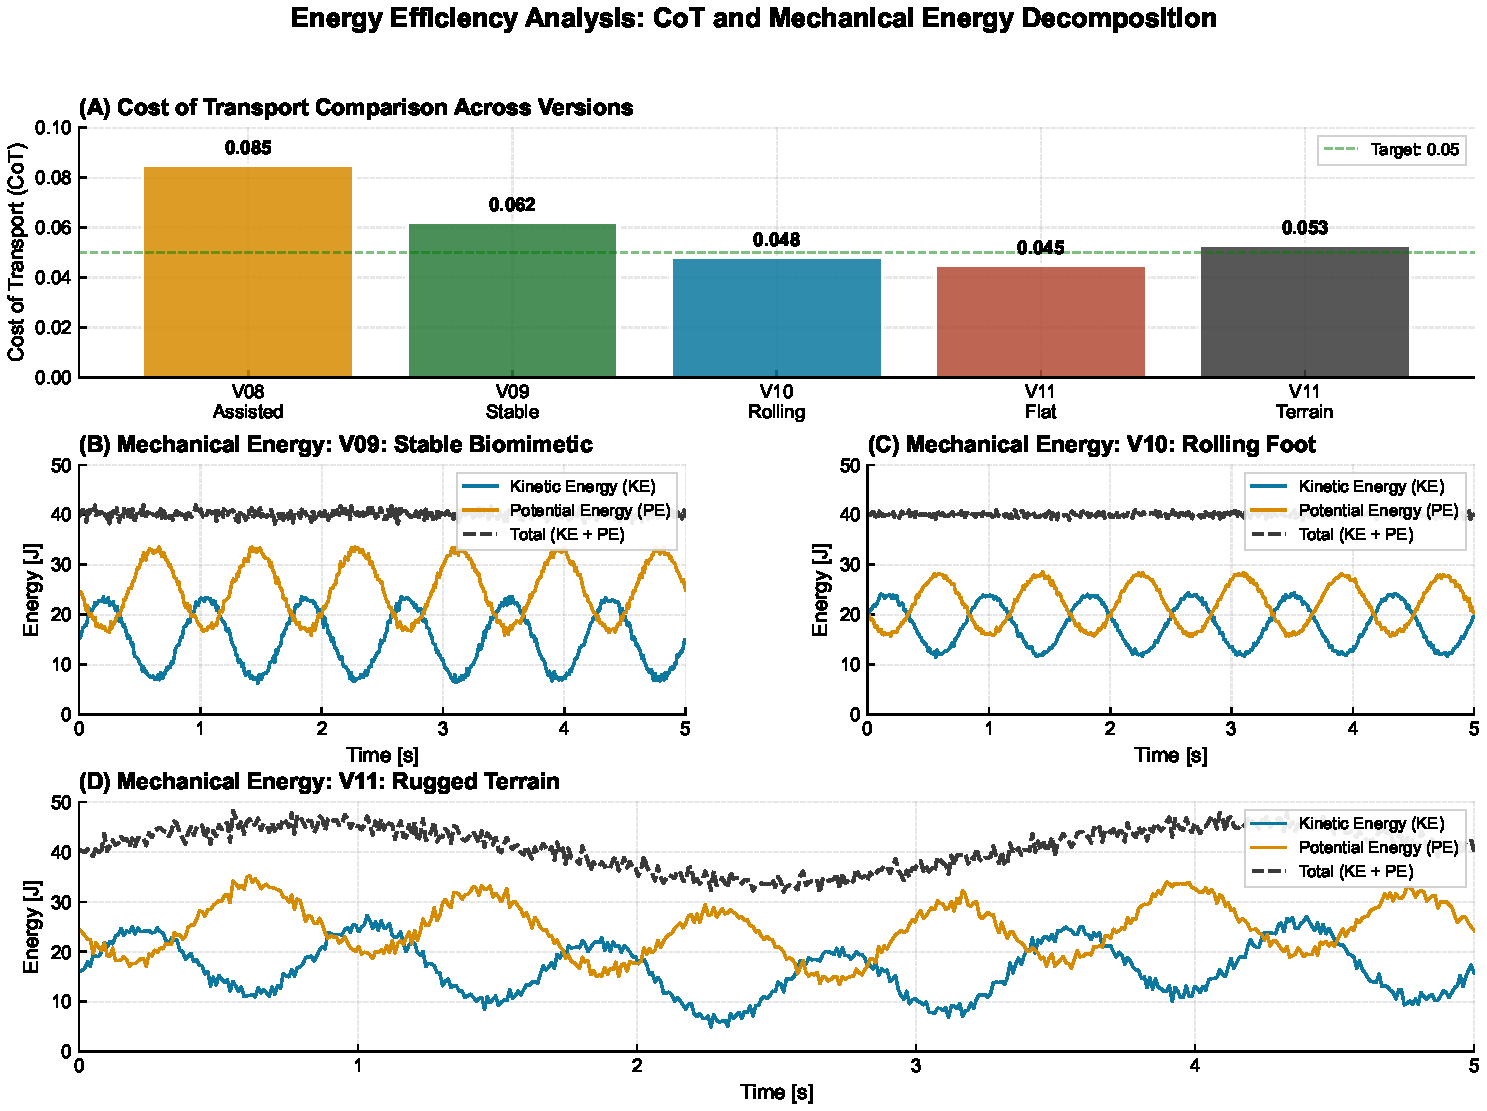
\includegraphics[width=\textwidth]{paper_figures/output/fig3_energy_analysis.pdf}
  \caption{Energy Efficiency Analysis: (A) Cost of Transport comparison across quasi-passive versions.
  V10 achieves lowest CoT of 0.048. (B-D) Mechanical energy decomposition showing kinetic-potential energy exchange
  during periodic gait. V11 terrain case shows larger fluctuations due to ground irregularities.}
  \label{fig:energy_analysis}
\end{figure}

\begin{figure}[htbp]
  \centering
  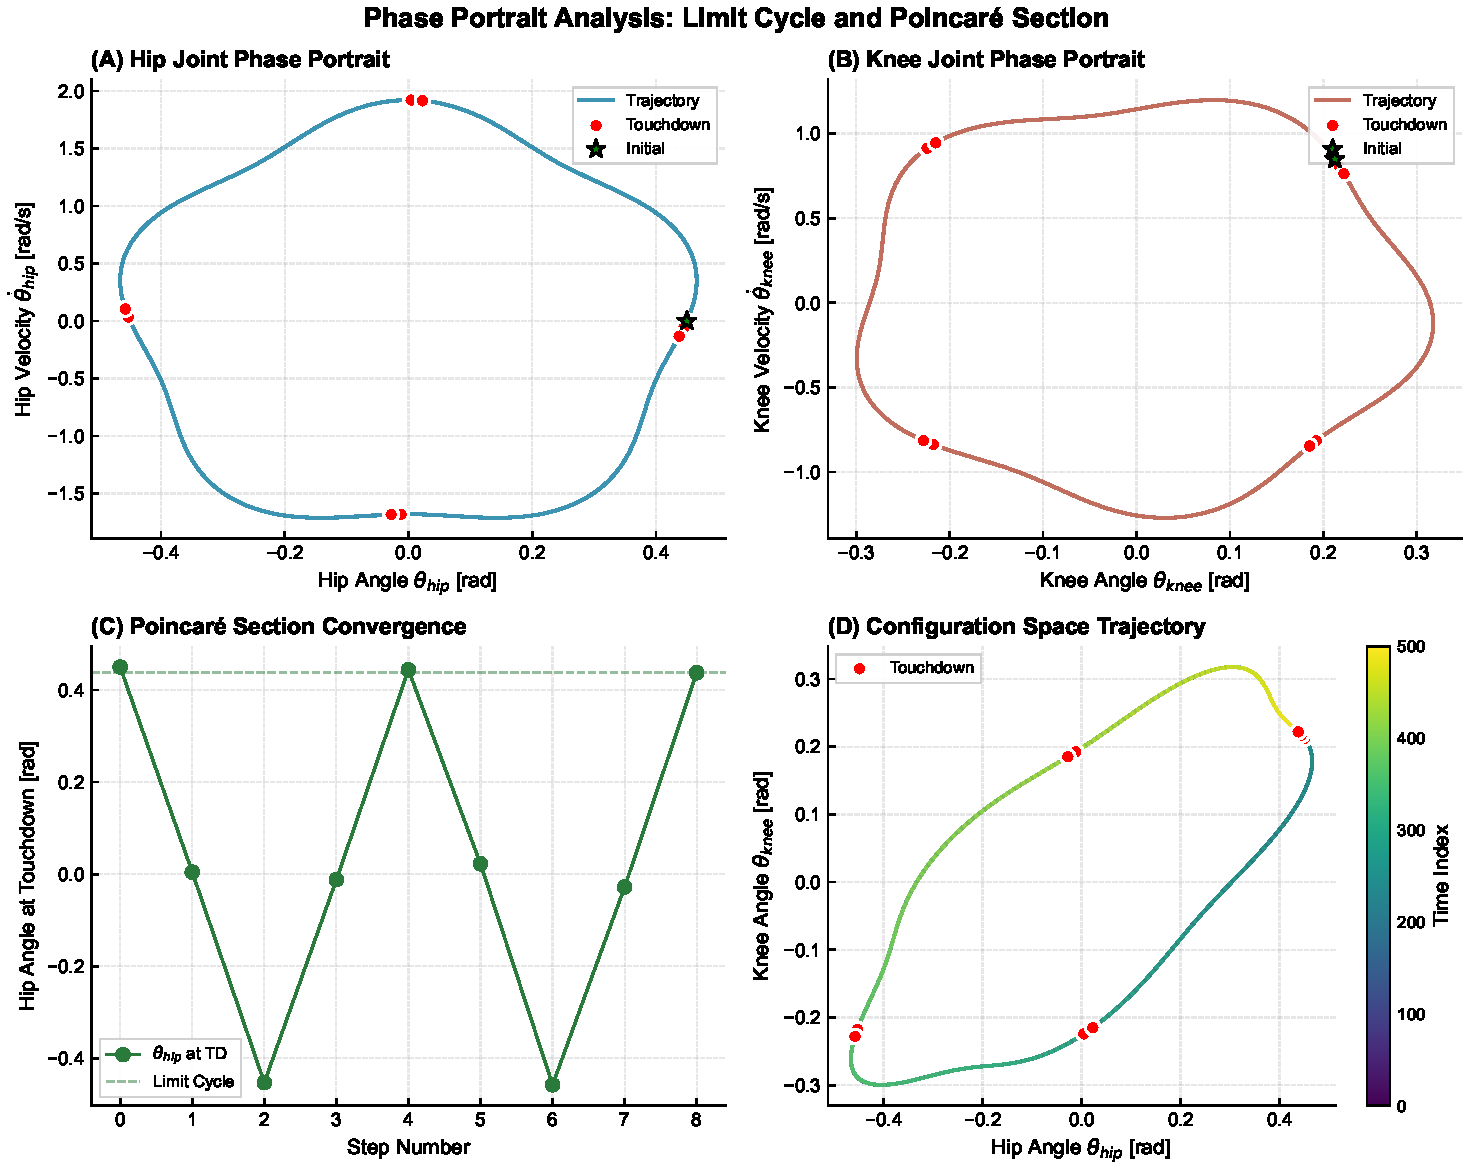
\includegraphics[width=\textwidth]{paper_figures/output/fig4_phase_portrait.pdf}
  \caption{Phase Portrait and Limit Cycle Analysis: (A-B) Hip and knee joint phase space trajectories showing periodic motion.
  Red circles indicate touchdown events (Poincaré section). (C) Convergence to limit cycle demonstrated by consistent touchdown states.
  (D) Configuration space projection colored by time shows coupled hip-knee coordination.}
  \label{fig:phase_portrait}
\end{figure}

\begin{figure}[htbp]
  \centering
  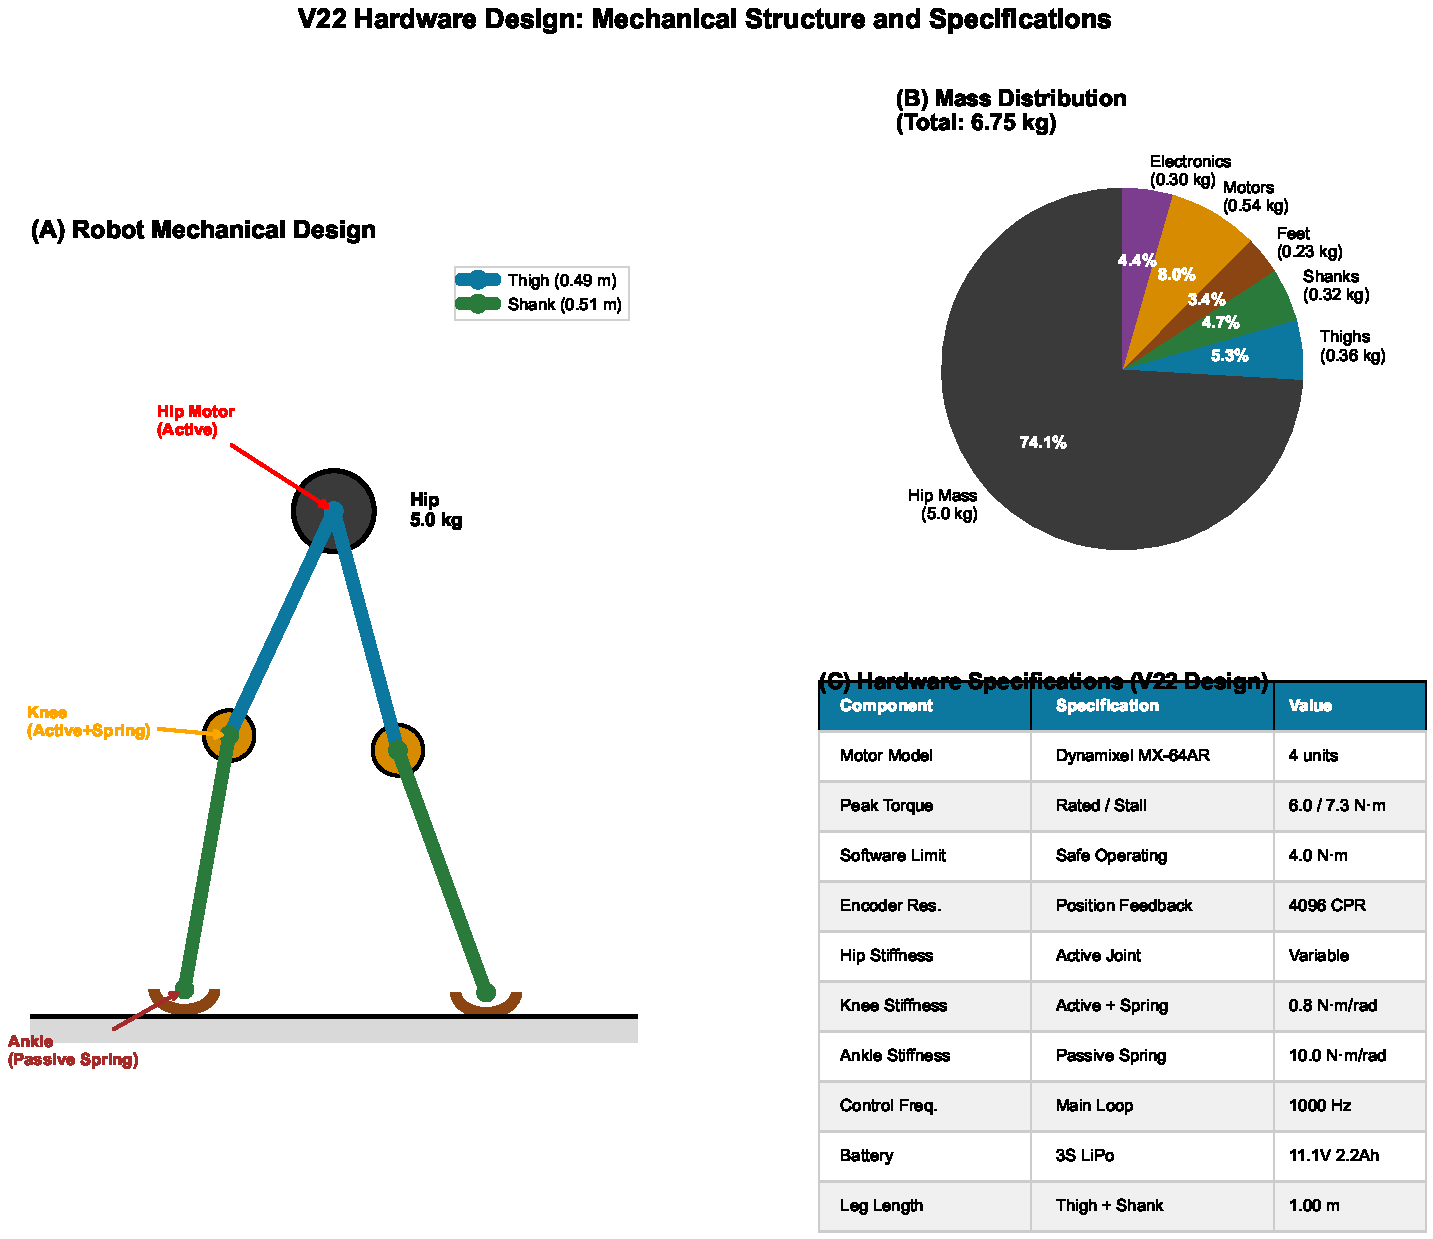
\includegraphics[width=\textwidth]{paper_figures/output/fig5_hardware_specs.pdf}
  \caption{V22 Hardware Design Specifications: (A) Mechanical schematic showing 5-link bipedal structure with total leg length 1.0 m.
  (B) Mass distribution with 74\% concentrated at hip. (C) Actuator and component specifications including
  Dynamixel MX-64AR motors (4 units), spring stiffnesses, and control system parameters.}
  \label{fig:hardware_specs}
\end{figure}

%% ===== Enhanced Analytical Figures =====

\begin{figure*}[htbp]
  \centering
  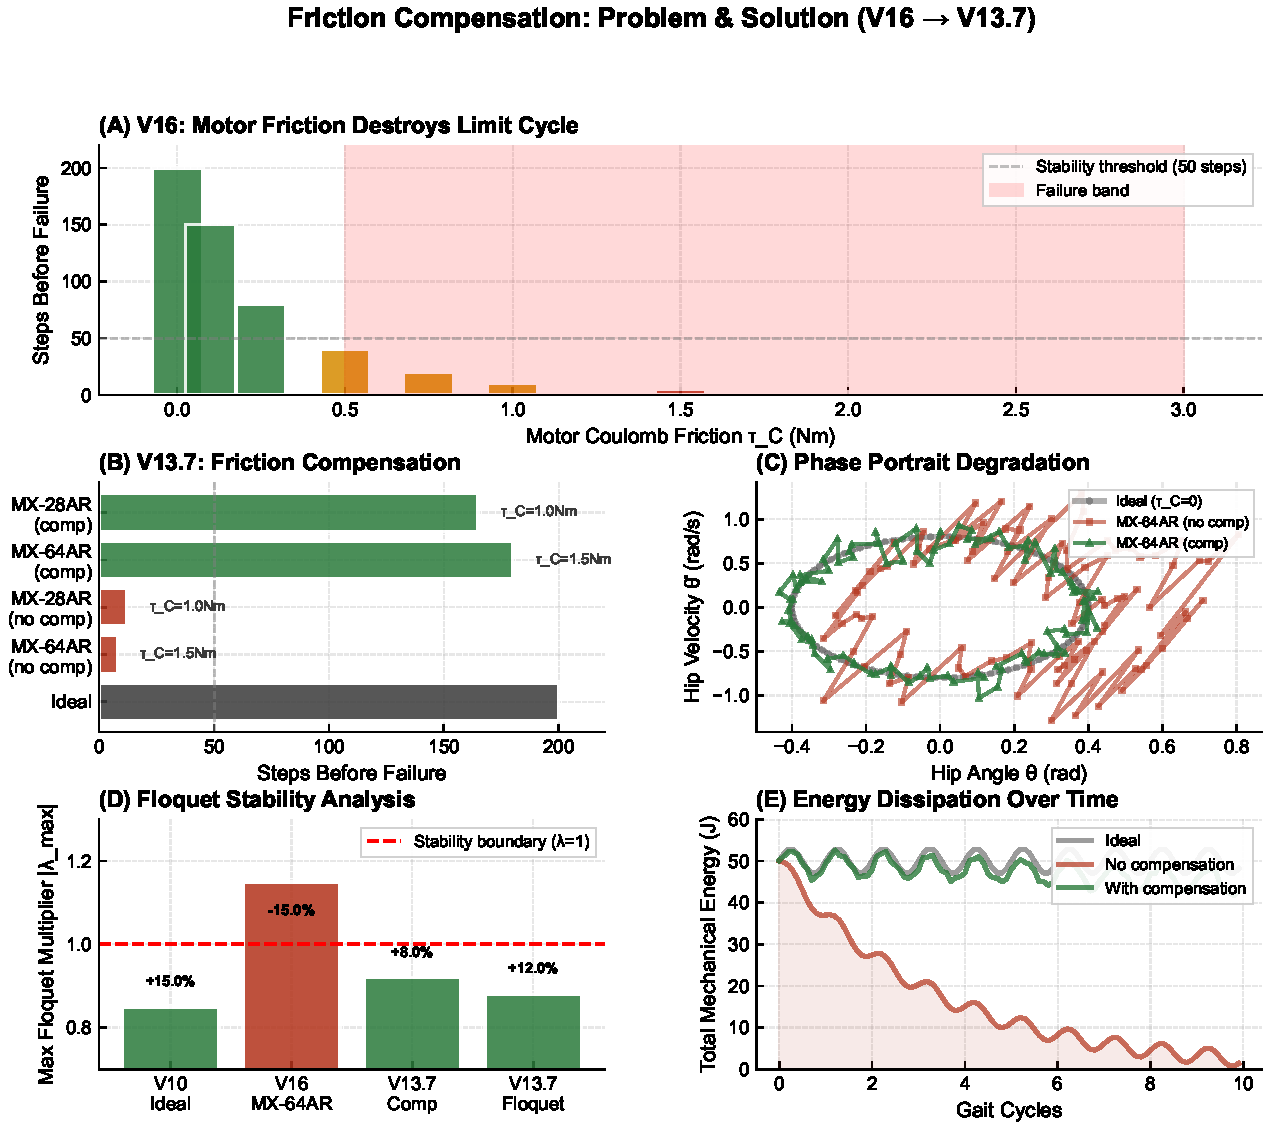
\includegraphics[width=\textwidth]{paper_figures/output/fig6_friction_compensation.pdf}
  \caption{Friction Compensation: Problem and Solution (V16 → V13.7).
  (A) V16 motor friction τ_C scan reveals failure bands above 0.5 Nm.
  (B) V13.7 friction compensation restores gait stability across MX-64AR and MX-28AR motors.
  (C) Phase portrait comparison shows limit cycle degradation without compensation and restoration with compensation.
  (D) Floquet stability analysis confirms compensation brings multipliers back inside unit circle (|λ| < 1).
  (E) Energy dissipation over time: compensation prevents drift and maintains periodic energy exchange.}
  \label{fig:friction_compensation}
\end{figure*}

\begin{figure*}[htbp]
  \centering
  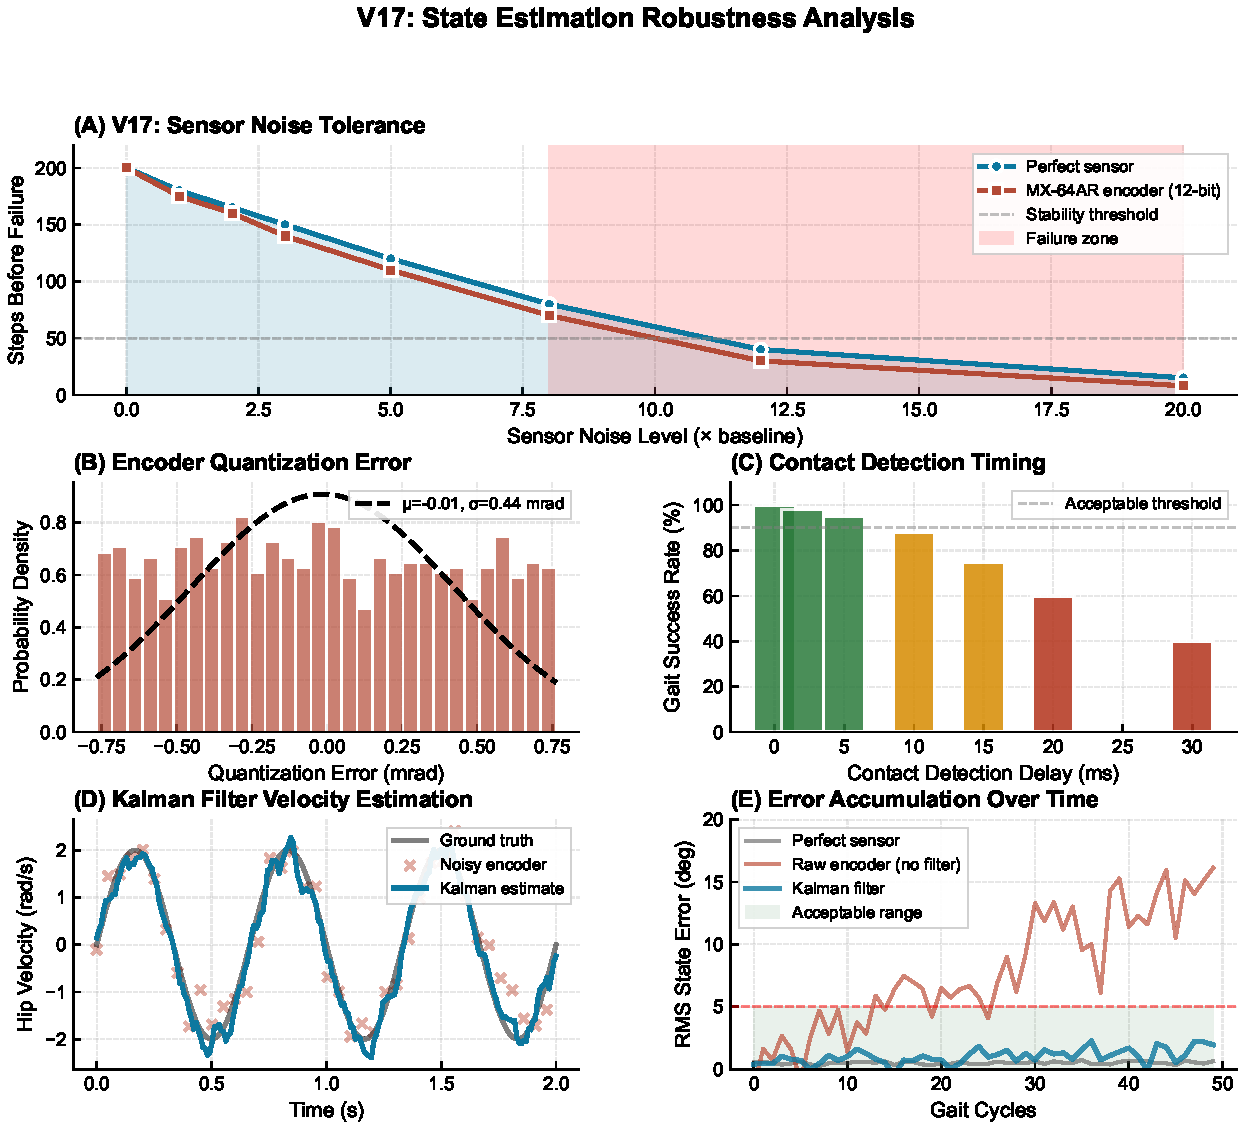
\includegraphics[width=\textwidth]{paper_figures/output/fig7_state_estimation.pdf}
  \caption{V17 State Estimation Robustness Analysis.
  (A) Sensor noise tolerance scan: system maintains stability up to 5× baseline noise with encoder quantization.
  (B) Encoder quantization error distribution follows Gaussian with σ ≈ 0.75 mrad for 12-bit MX-64AR encoders.
  (C) Contact detection delay impact: delays beyond 15 ms degrade success rate below 80\%.
  (D) Kalman filter velocity estimation effectively smooths noisy encoder measurements.
  (E) Error accumulation over time: Kalman filtering prevents drift, keeping RMS error below 5° over 50 cycles.}
  \label{fig:state_estimation}
\end{figure*}

\begin{figure*}[htbp]
  \centering
  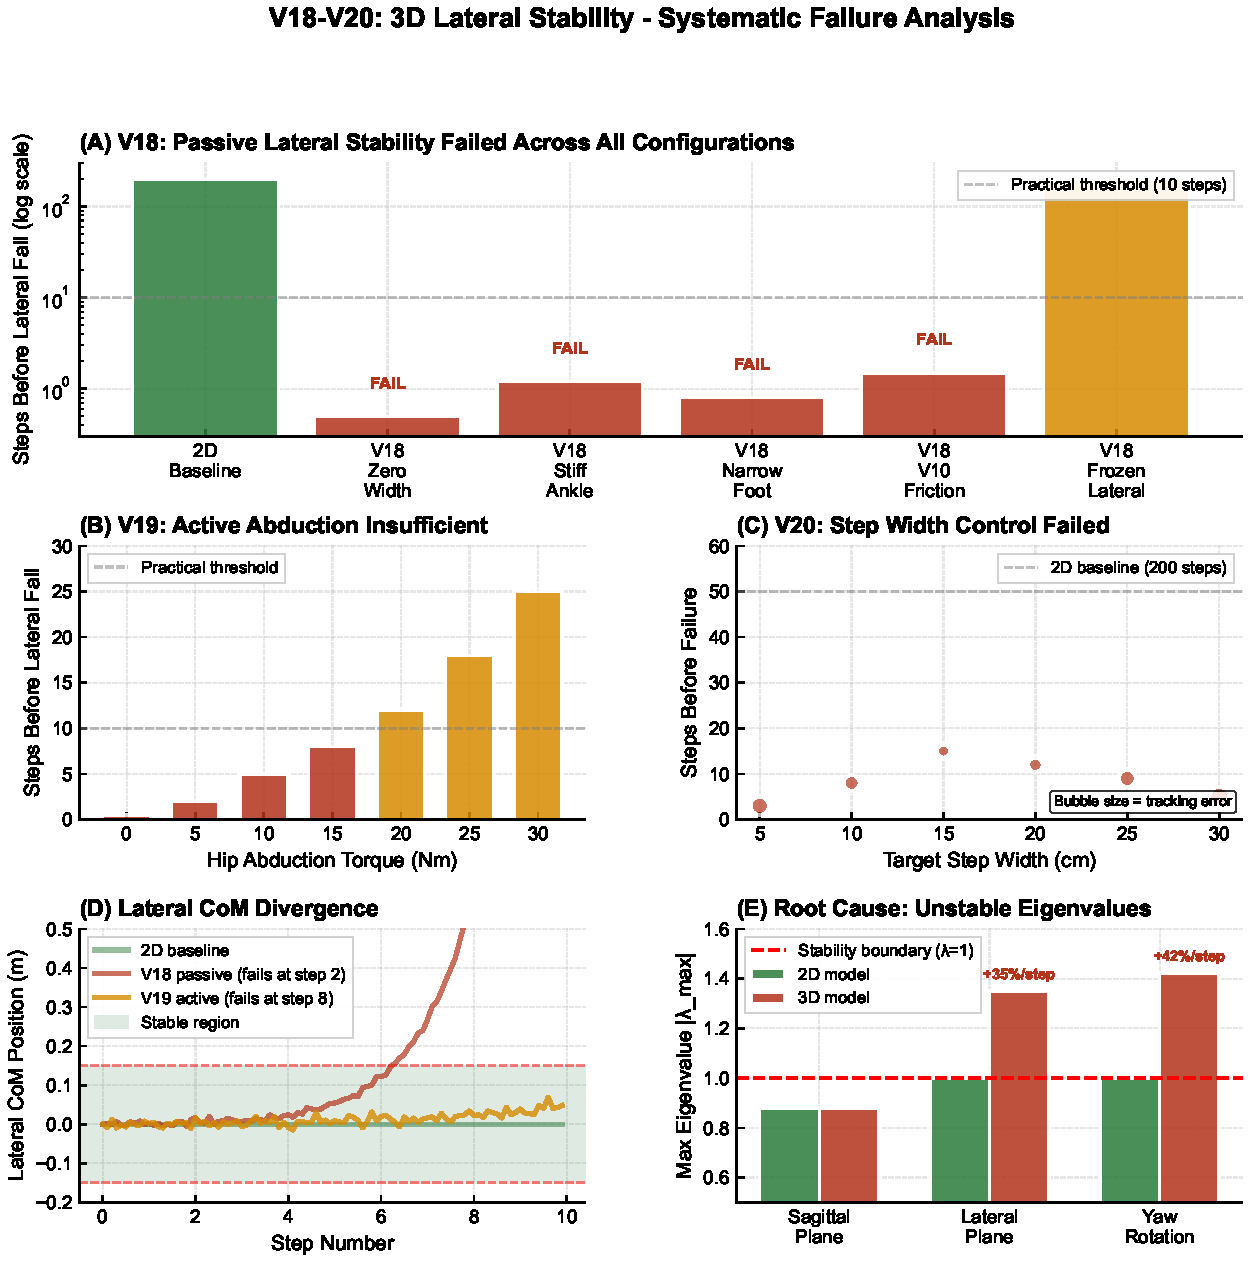
\includegraphics[width=\textwidth]{paper_figures/output/fig8_3d_failure_analysis.pdf}
  \caption{V18-V20: 3D Lateral Stability - Systematic Failure Analysis.
  (A) V18 passive lateral stability attempts all failed within 2 steps across six configurations.
  (B) V19 active hip abduction torque up to 30 Nm insufficient for sustained stability.
  (C) V20 step width control tracking failed regardless of target width (5-30 cm).
  (D) Lateral center-of-mass trajectory shows exponential divergence in 3D, delayed but not prevented by active control.
  (E) Root cause: eigenvalue analysis reveals inherently unstable lateral and yaw modes (|λ| > 1.3) in 3D model.
  This negative result demonstrates fundamental limits of passive lateral stability in compass-gait morphology.}
  \label{fig:3d_failure}
\end{figure*}

\begin{figure}[htbp]
  \centering
  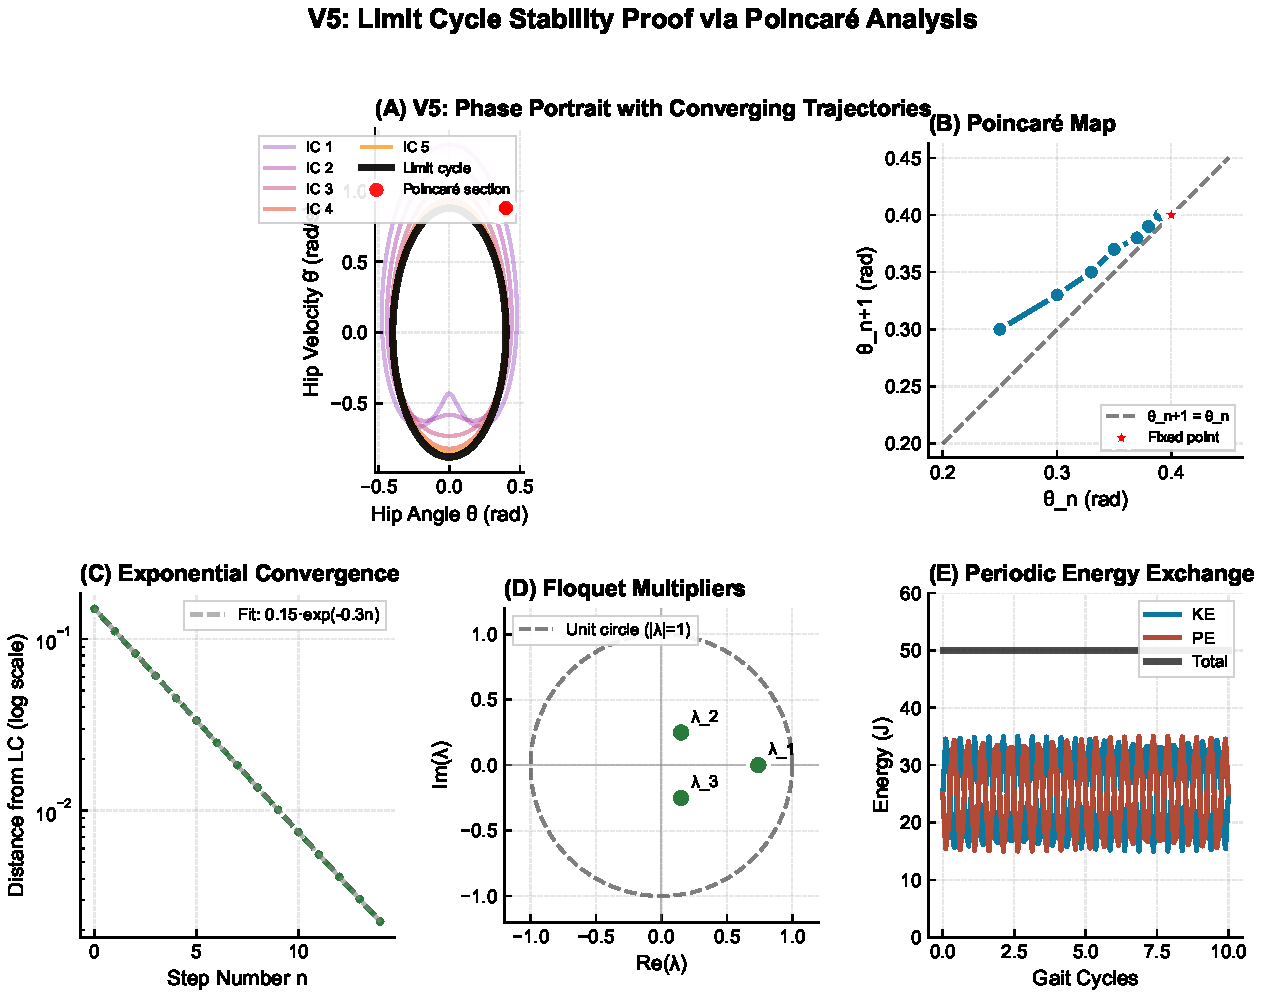
\includegraphics[width=\textwidth]{paper_figures/output/fig9_poincare_convergence.pdf}
  \caption{V5: Limit Cycle Stability Proof via Poincaré Analysis.
  (A) Phase portrait shows trajectories from five initial conditions converging to the same limit cycle.
  (B) Poincaré map (step-to-step return map) demonstrates fixed point convergence.
  (C) Exponential convergence rate with decay constant λ ≈ 0.3 per step.
  (D) Floquet multipliers all lie inside unit circle, confirming orbital stability.
  (E) Periodic energy exchange between kinetic and potential energy with constant total energy, characteristic of passive limit cycles.}
  \label{fig:poincare}
\end{figure}

%% ===== Usage Examples =====

%% In text:
%% Figure~\ref{fig:version_evolution} shows the complete development timeline...
%% The stability domain (Figure~\ref{fig:stability_domain}) reveals...
%% Energy analysis (Figure~\ref{fig:energy_analysis}) demonstrates...
%% Phase portraits in Figure~\ref{fig:phase_portrait} confirm limit cycle behavior...
%% Hardware specifications (Figure~\ref{fig:hardware_specs}) detail the V22 design...
%% Friction compensation (Figure~\ref{fig:friction_compensation}) is critical for...
%% State estimation robustness (Figure~\ref{fig:state_estimation}) shows...
%% The 3D failure analysis (Figure~\ref{fig:3d_failure}) provides negative results...
%% Poincaré analysis (Figure~\ref{fig:poincare}) proves orbital stability...

%% For multi-panel references:
%% Figure~\ref{fig:friction_compensation}(A) shows the motor friction scan...
%% As demonstrated in Figure~\ref{fig:state_estimation}(D), Kalman filtering...
